\documentclass[main.tex]{subfiles}
\begin{document}
	
	\chapter{Perception}
		\chapterauthor{Author}
		
		\section{General}
		The main changes and improvements upon the status presented at milestone 1 are the following: Perception now runs inside an actionserver, in contrast to 				plain robosherlock. Additionally, Caffe is now used for feature extraction, and KNN is used for the classification of detected objects. Also, image data of 		available objects was recorded, which was then used for classification purposes.
		
		\section{Actionserver}
			\subsection{Interfaces}
			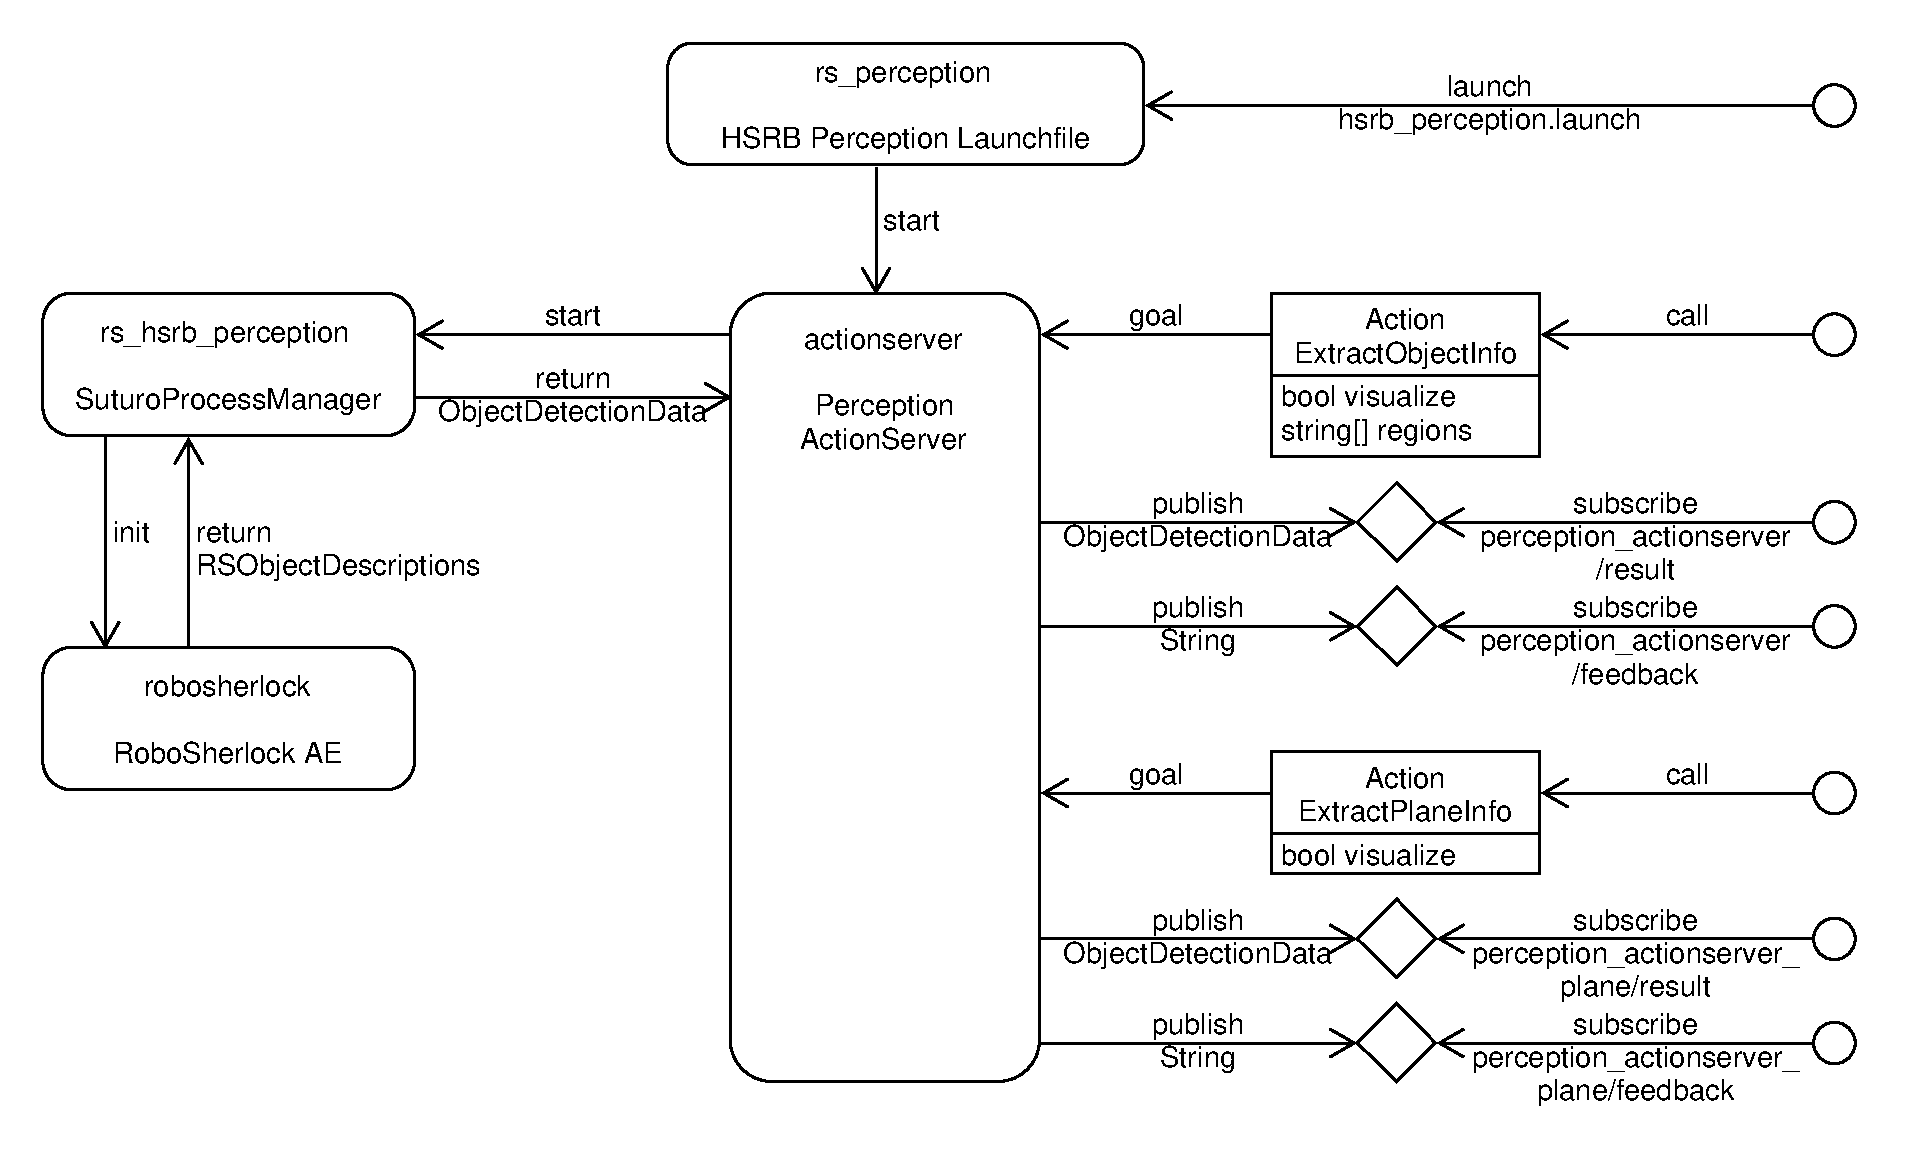
\includegraphics[width=\textwidth]{../architecture/perception_architecture/perception.pdf}
			
			\subsection{Packages}
			\subsubsection{actionserver}
			Implements the "ExtractObjectInfo" and "ExtractPlaneInfo" action servers and the corresponding action clients.
			Internally the "SuturoProcessManager" from "rs\_hsrb\_perception" is used to communicate with RoboSherlock.
			The action server invokes "SuturoProcessManager::run()" with the given parameters. 

			\subsubsection{rs\_perception}
			Includes launch-, configuration- and analysis descriptor files.
			In order to start the perception action servers you have to call:\\
			"roslaunch rs\_perception hsrb\_perception.launch"\\
			To convert published URDFs to YAML run: "region\_filter\_setup.py" (originally from Suturo1819).\\
			Generated YAML map descriptors must be placed in the "config" folder.

			\subsubsection{rs\_hsrb\_perception (forked from suturo1819)}
			Implements a RoboSherlock process manager "SuturoProcessManager".
			The manager gets called from the "actionserver" and executes the selected pipeline once.
			
			In order to perceive objects that are placed on the ground, the SuturoRegionFilter gets reconfigured
			to disable the region filtering. Set the region parameter to \{ "robocup\_default" \} to enable this feature.

		\section{Classification}
		    \subsection{Feature Extraction}
		    In order to gain features on which to train classifiers, Caffe\footnote{\url{https://caffe.berkeleyvision.org/}}, in combination with the robosherlock 				package rs\_addons\footnote{\url{https://github.com/bbferka/rs_addons}} is used. rs\_addons was forked, off of another fork\footnote{\url{https://					github.com/Vanessa-rin/rs_addons}} to be able to make changes to the source code\footnote{\url{https://github.com/Jastock/rs_addons/tree/								rs_classifier_makeover}}.\\
		    
		    rs\_addons provides a program called "featureExtractor". It needs a split file, which specifies the classes your classifier will later output, as well 				as an output folder and the caffemodel to use as inputs. To make this process easier, shell scripts to generate a split file and a classlist from 					directory names can be found in \url{https://github.com/SUTURO/suturo_perception/tree/master/featureExtraction/tools}. Training images have to be 					provided as well, which have to be placed in the "object\_data" folder in the rs\_resources\footnote{\url{https://github.com/RoboSherlock/							rs_resources}} package. More information on how the training images can be recorded will be provided in the "Recording of images" section.\\
		    
		     Running this program will provide a file containing a matrix with features for every class specified in the split file. It also provides a file with a 			mapping from the classnames to the numbers used in the feature matrix to represent the classes. These files can now be used to train classifiers. For 				exact information on how to do feature extraction using this method, refer to \url{https://github.com/SUTURO/suturo_perception/blob/master/							featureExtraction/featureExtraction.md}. 
			
			\subsection{Classifiers}
			The newly generated files from the previous section can then be used in the annotators for classification provided by rs\_addons. Until now, the KNN-					Annotator was used for classification. The SVM-Annotator and the RF-Annotator were tested to make sure they work, but to use them effectively, their 					settings have to be tweaked.\\
			
			To find out which of these methods for classification works best for this specific problem, they have to be objectively compared. Up to this point, 					there is no effective way of doing this. The implementation of such a way is a goal for the next milestone. The idea is to implement a tool that 						can be used to label the objects in an example scene. A different tool can then run classification algorithms on these labeled scenes and calculate 					evaluation criteria, such as accuracy, recall, precision and the f-score. The tool should also be able to evaluate the speed of the algorithms. On the 				basis of these criteria, the algorithms can be objectively compared and the best one for the problem at hand can be selected.
			
			\subsection{KNN Confidence}
			In the official version of rs\_addons the confidence for a prediction is calculated by only looking at the distance of the first neighbor to the new 					sample. This is not a sufficient representation and it does not show difference when choosing different K's. To fix this, a new version of the 						confidence was implemented by dividing the number of neighbors belonging to the result class by the total number of neighbors, in other words the K.
			The new version can be found in \url{https://github.com/Jastock/rs_addons/blob/rs_classifier_makeover/src/classifiers/RSKNN.cpp}, in the 								"calculateConfidence" function.  
			
			\subsection{Saving the classification results}
			To be able to compare and visualize the classification results, the classificationEvaluation package was implemented. It provides an actionclient, that 			sends action goals to the perception actionserver and receives the results. These results can be represented in a markdown table or plotted in a 						scatterplot. By leaving the "rsClassificationEvalutator" node running and stopping the actionserver to alter the configuration, different K's can be 					tested and saved in case of using KNN. The package can be found here: . 
		
		
		\section{Recording of images}  

\end{document}
